\RequirePackage{luatex85}
\documentclass[tikz]{standalone}

\usetikzlibrary{arrows,calc,fit,patterns,positioning,backgrounds,shapes}

\usepackage{fontspec}
\setmainfont{Source Sans Pro}

\tikzset{
  >=latex,
  every path/.style={
    shorten <=2pt,shorten >=2pt,>=stealth
  },
  background rectangle/.style={fill=white},
  component/.style={
    draw, rounded corners,
    text depth=0pt,
    minimum width=30mm,
    minimum height=10mm
  },
  db/.style={
    cylinder, shape aspect=.5, shape border rotate=90, draw,
    text depth=0pt,
    minimum width=30mm
  },
  onarrow/.style={
    font=\footnotesize
  },
  wrapper/.style={
    dashed,draw=black!70!white,rounded corners,inner sep=3mm
  },
  wrapperlabel/.style={
    fill=white,font=\scriptsize,
    text depth=0pt,
    anchor=west,
    xshift=-2mm
  },
  box/.style={
    draw=black!30!white,line width=2pt,rounded corners,inner sep=3mm
  },
  boxlabel/.style={
    fill=white,font=\small,
    text depth=0pt,
  }
}



\begin{document}

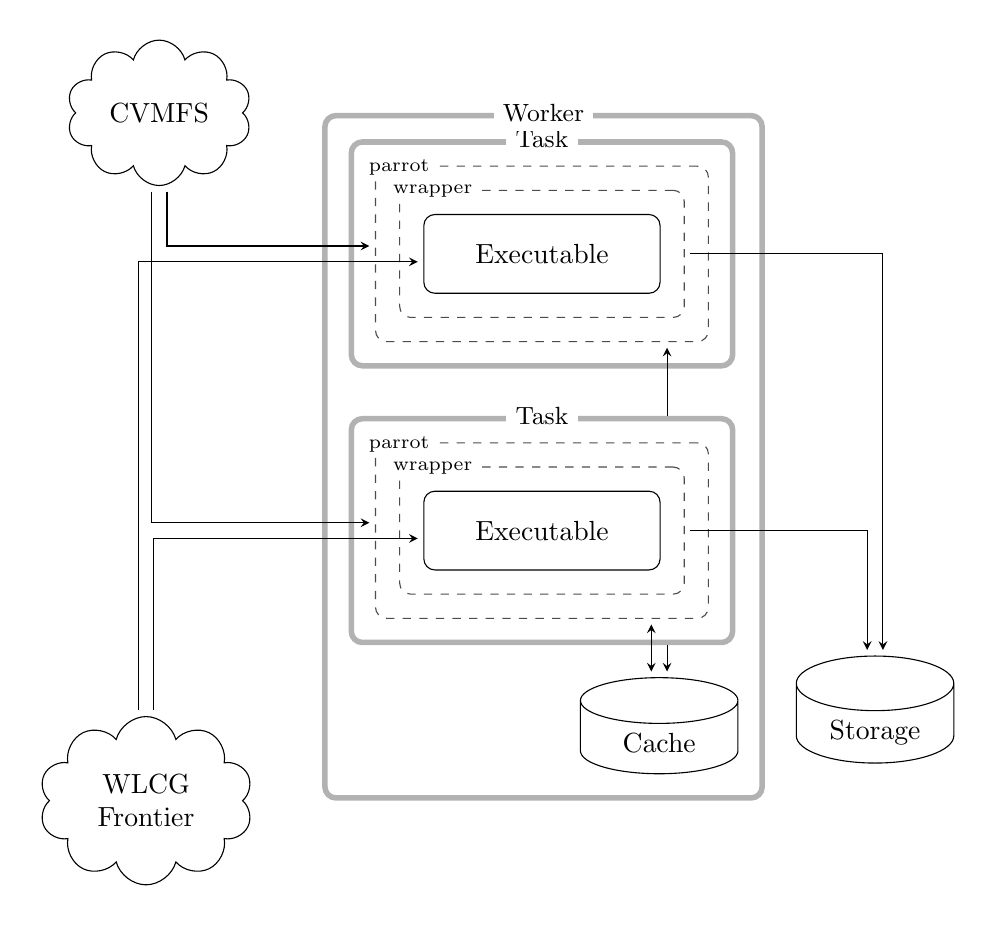
\begin{tikzpicture}[show background rectangle]
  \node[component] (e1) {Executable};
  \node[wrapper,fit=(e1)] (w1) {};
  \node[wrapper,fit=(w1)] (p1) {};

  \node[wrapperlabel] at (w1.north west) {wrapper};
  \node[wrapperlabel] at (p1.north west) {parrot};

  \node[box,fit=(p1)] (t1) {};
  \node[boxlabel] at (t1.north) {Task};

  \node[component,below=25mm of e1] (e2) {Executable};
  \node[wrapper,fit=(e2)] (w2) {};
  \node[wrapper,fit=(w2)] (p2) {};

  \node[wrapperlabel] at (w2.north west) {wrapper};
  \node[wrapperlabel] at (p2.north west) {parrot};

  \node[box,fit=(p2)] (t2) {};
  \node[boxlabel] at (t2.north) {Task};

  % \node[component] (t1) {Task};
  % \node[component,below=5mm of t1] (t2) {Task};

  \node[db,minimum width=20mm,below right=5mm and 7.5mm of t2.south] (cache) {Cache};
  \coordinate (c1) at ($(cache.north) + (1mm,0)$);
  \coordinate (c2) at ($(cache.north) - (1mm,0)$);
  \draw[<-,shorten >=0pt] (c1) -- (c1 |- t2.south);
  \draw[->,shorten <=0pt] (c1 |- t2.north) -- (c1 |- p1.south);
  \draw[<->] (c2) -- (c2 |- p2.south);

  \node[box,fit=(t1)(t2)(cache)] (worker) {};
  \node[boxlabel] at (worker.north) {Worker};

  \node[draw,cloud,aspect=1.5,left=of worker.north west] (cvmfs) {CVMFS};
  \node[draw,cloud,aspect=1.5,text width=15mm,align=center,left=of worker.south west] (wlcg) {WLCG\\Frontier};

  \draw[->] ($(cvmfs.south) + (1mm,0)$) |- ($(p1.west) + (0,1mm)$);
  \draw[->] ($(cvmfs.south) - (1mm,0)$) |- ($(p2.west) + (0,1mm)$);

  \draw[->] ($(wlcg.north) - (1mm,0)$) |- ($(e1.west) - (0,1mm)$);
  \draw[->] ($(wlcg.north) + (1mm,0)$) |- ($(e2.west) - (0,1mm)$);

  \node[db,minimum width=20mm,above right=5mm and 10mm of worker.south east] (storage) {Storage};
  \draw[->] (w1) -| ($(storage.north) + (1mm,0)$);
  \draw[->] (w2) -| ($(storage.north) - (1mm,0)$);
\end{tikzpicture}

\end{document}
